\chapter{Fehlerfortpflanzung in modularen Anlagen durch Einsatz von Graphen}\label{ch:ffpflMod}
Im Kapitel \ref{ch:fehlerfortpfl} werden verschiedene Methoden der \acf{fdi} hinsichtlich einer Verwendbarkeit f\"ur die Untersuchung von modularen Anlagen bewertet. Die vorgestellten Methoden werden dazu in drei Kategorien eingeteilt, welche sich ma\ss{}geblich hinsichtlich der Informationen unterscheiden, welche zur Anwendung der Methoden notwendig sind. Im Kontext der vorliegenden Arbeit wird davon ausgegangen, dass die Beschreibung einzelner Module, die \ac{hazop}"=Studien der Module und eine Beschreibung der modularen Gesamtanlage vorliegt. Das vorhandene Wissen besteht also aus Expertenwissen und Informationen \"uber die Kopplung der Module. Das vorhandene Wissen umfasst also keinerlei Messdaten, weswegen die im Abschnitt \ref{sec:fAna_dat} vorgestellten datenbasierten Verfahren der \ac{fdi} als ungeeignet bewertet werden. \newline
Die im Abschnitt \ref{sec:fAna_modQuant} vorgestellten quantitativen modellbasierten Verfahren ben\"otigen ein geeignetes quantitatives Modell der Gesamtanlage. Die Erstellung dieser Modelle ist aufwendig und m\"ogliche Zeiteinsparungen daher gering, die Wiederverwendbarkeit limitiert und die Nutzung von vorhandenem Wissen \"uber die einzelnen Module kompliziert. Daher werden auch diese Methoden als nicht geeignet eingestuft. \newline
Im Abschnitt \ref{sec:fAna_modQual} werden die modellbasierten qualitativen Verfahren vorgestellt. Diese nutzen a priori vorhandenes Wissen \"uber den betrachteten Prozess und entwickeln darauf aufbauend ein Modell des Systemverhaltens. Diese Art von Wissen wird im Rahmen der vorliegenden Arbeit als vorhanden angenommen. Die erfolgreiche Nutzung von Expertenwissen zur Analyse von Fehlerfortpflanzungen wird im Abschnitt \ref{sec:fAna_automatHazop} anhand zahlreicher Verfahren zur Automatisierung von \acp{hazop} dargelegt. Die vorgestellten Methoden der qualitativen modellbasierten \ac{fdi} werden als prinzipiell geeignet bewertet, um die Fehlerfortpflanzung von Prozessabweichungen innerhalb modularer Anlagen zu untersuchen, da diese Methoden im industriellem Ma\ss{}stab durch Einsatz von wiederverwendbarem Detailwissen erfolgreich f\"ur Fehlerfortpflanzungsbetrachtungen eingesetzt wurden. \newline
Derzeit existieren noch keine bekannten Verfahren, welche direkt f\"ur aus Modulen bestehende Anlagen eingesetzt werden k\"onnen. Problematisch ist die Beschreibung des Auswirkungen einer Kopplung der Module und die konkrete Verwendung des \"uber die einzelnen Module vorhandenen Wissens. In diesem Kapitel wird die Anwendung von gerichteten Graphen skizziert, um dieses Problem zu l\"osen. Die Anwendung anderer modellbasierter qualitativer Verfahren ist m\"oglich und sollte gezielt untersucht werden. Gerichtete Graphen sind die allgemeine Form von \acf{sdg}. Deren Verwendung ist besonders weit verbreitet und es existieren zahlreiche Softwares zur Computer"=gest\"utzten Implementierung. Ein kostenloses Werkzeug ist auf der Website \url{http://www.graphviz.org/} zu beziehen. Hier wird jedoch eine Implementierung mit Hilfe von Matlab Simulink\textsuperscript{\textregistered} durchgef\"uhrt, da dieses Werkzeug besonders weit in der Industrie verbreitet ist. \newline
Die Verwendung von Graphen bietet die M\"oglichkeit einer teil automatisierten Erstellung, allerdings wird das Ergebnis weder plausibilisiert noch bildet es zeitliche Zusammenh\"ange ab {(vgl. \cite{Yang_2010})}. Der Einsatz von Gewichten macht eine Bewertung der Wahrscheinlichkeiten von Fehlerfortpflanzungen m\"oglich, diese M\"oglichkeit bleibt in der vorliegenden Arbeit aber ungenutzt, da kein Wissen \"uber konkrete Wahrscheinlichkeiten vorhanden ist. Statt dessen wird im folgenden Abschnit \ref{sec:graphHazop} gezeigt, wie auf Basis von \ac{hazop}"=Studien einzelner Modelle Graphen erzeugt werden k\"onnen, welche die bereits analysierten Wechselwirkungen abbilden. Anschlie\ss{}end wird im Abschnitt \ref{sec:kopplung} dargelegt, wie die bekannte Kopplung der Module zu einer Gesamtanlage zum Verbinden dieser Graphen genutzt werden kann. Der so entstehende Gesamtgraph wird dann auf die Beschreibung von modul\"ubergreifenden Wechselwirkungen hin untersucht. 

\section{Algorithmus zur Erstellung von gerichteten Graphen auf Basis von HAZOP"=Studien}\label{sec:graphHazop}
Die Auswertung von textbasierten Informationen durch Software ist besonders gut geeignet, wenn diese Informationen strukturiert sind. Dazu ist die Verwendung einer Ontologie sinnvoll. Hier wird die Analyse einer modularisierten Ethylacetatanlage nach \cite{Pfeffer_2016, Pfeffer_2017} genutzt, welche nicht derart strukturiert ist. Im Folgenden wird ein Modul bestehend aus Zulauf, Tank mit R\"uhrer und Pumpe im Ablauf betrachtet, welches in \figureref{fig:PIDMod1} abgebildet ist. Die dazu vorliegende \ac{hazop} ist in \tabref{tab:hazopBsp_M1} zu finden. Betrachtet werden die physikalischen Gr\"o\ss{}en Fluss und F\"ullstand. Deren Wechselwirkung soll durch einen Graphen basierend auf der vorhandenen \ac{hazop} dargestellt werden.  

Da der zu konstruierende Graph auf der \ac{hazop} basieren soll, m\"ussen die vorhandenen Informationen geeignet verarbeitet werden. Dazu dient die Funktion \glqq buildGraphForModule\grqq { }. Sie liest aus einem bestimmten Bereich eines w\"ahlbaren Arbeitsblattes einer spezifizierten Excel Datei die Daten aus. Die Daten werden anschlie\ss{}end analysiert. \newline
Im ersten Schritt werden die Variablen F\"ullstand und Fluss durch die Buchstaben L und F respektive ersetzt und mit einer Zahl kombiniert, welche die Nummer des analysierten Moduls widerspiegelt. Weiterhin wird diese Abk\"urzung mit dem in der Spalte \glqq unit\grqq { }definierten Text kombiniert. Das Ergebnis wird im Graphen als Knoten dargestellt. Der Eingangsstrom wird durch den Knoten \textit{in1F1}, der Ausgangsstrom durch den Knoten \textit{out1F1} und der F\"ullstand im Tank mit Hilfe des Knotens \textit{tankL1} abgebildet. \newline
Im zweiten Schritt werden die Auswirkungen von Abweichungen betrachtet. Diese k\"onnen entweder auf Prozessvariablen im Modul, auf externe Variablen oder auf Equipment wirken. Da in der Implementierung nur Durchfluss und F\"ullstand betrachtet werden, ist eine Wirkung auf andere als diese Gr\"o\ss{}en in der Verarbeitung gleichbedeutend mit einer Wirkung auf Equipment. Solche Auswirkungen werden durch spezielle Knoten dargestellt, welche durch den Buchstaben \textit{C} und eine Zahlenkette identifiziert werden. In \figureref{fig:graph_mod1} wird das Ergebnis der Graphenbildung f\"ur das Tankmodul 1 dargestellt.

\begin{figure}[h!tb]
\centering
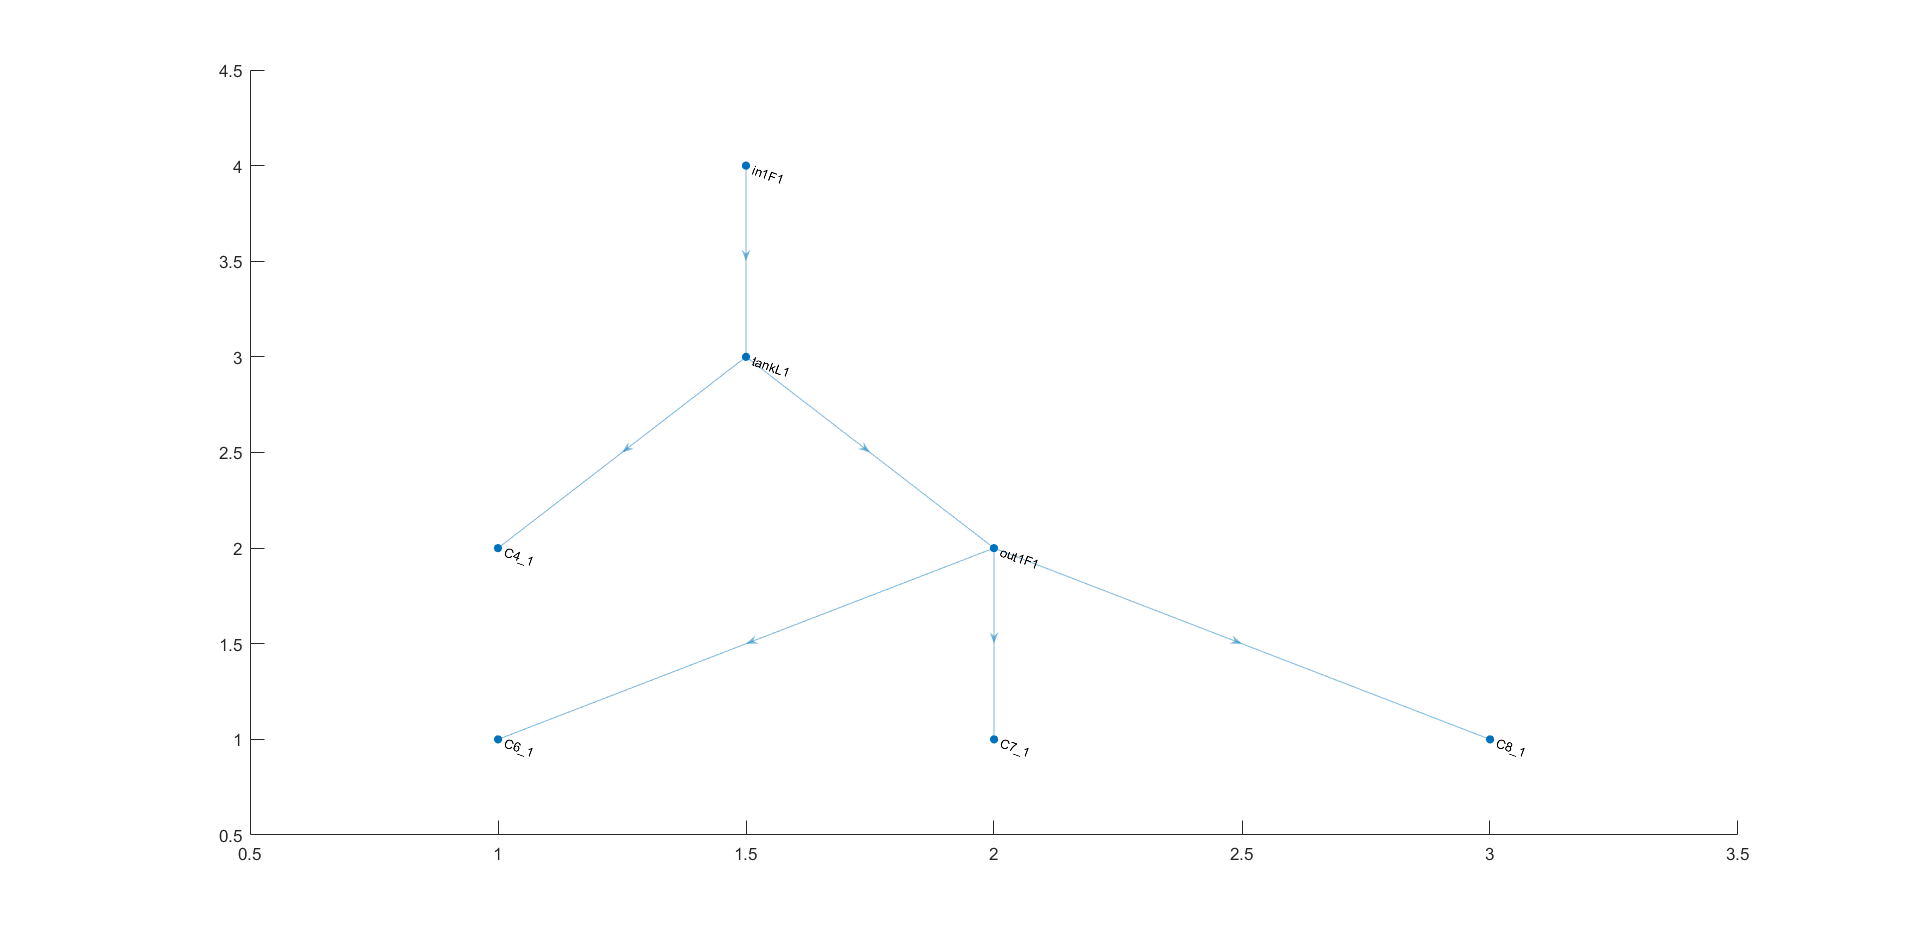
\includegraphics[width=\textwidth]{bilder/04_code_Modul1.png}
\caption[Digraph von Modul 1]{Digraph von Tankmodul 1 auf Basis der HAZOP}
\label{fig:graph_mod1}
\end{figure}

In \figureref{fig:graph_mod1} ist beispielsweise die Auswirkung vom Eingangsstrom auf das Tankvolumen und dessen Wirkung auf den Rest des Moduls dargestellt. Entsprechend der in \tabref{tab:hazopBsp_M1} dargestellten \ac{hazop} hat der Stoffstrom vom Eingang je nach betrachteter Abweichung verschiedene Auswirkungen auf das Tankvolumen. Diese m\"oglichen Auswirkungen k\"onnen mit Hilfe der Funktion \glqq findConsequenceOfDeviation\grqq { }ermittelt werden. Diese Funktion liefert alle Auswirkungen auf einen betrachteten Knoten, welche durch Abweichungen von benachbarten Knoten entstehen k\"onnen. F\"ur den Knoten \textit{tankL1} liefert die Funktion daher die m\"oglichen Auswirkungen \textit{less{\_}tankL1, more{\_}tankL1, less{\_}tankL1}. Dies entspricht den in \tabref{tab:hazopBsp_M1} untersuchten Fehlerf\"allen mit der ID $1-3$. \newline
Der Knoten \textit{C4{\_}1} repr\"asentiert eine Auswirkung auf ein Equipment. Die Anwendung der Funkton \glqq findConsequenceOfDeviation\grqq { }auf diesen Knoten liefert die Information, dass es sich um die Auswirkung \glqq more pressure\grqq { }handelt. Durch Anwendung der Funktion \glqq findDeviationforConsequence\grqq { }ergibt sich, dass die Abweichung, welche zu dieser Auswirkung gef\"uhrt hat, \glqq more tankL1\grqq { }ist. Als Ursache f\"ur diese Abweichung kann mit Hilfe von \glqq findCauseForDeviation\grqq { }die Information \glqq ID=2\grqq { }ermittelt werden. Die M\"oglichkeit eines Sensorfehlers als Ursache f\"ur die Abweichung \glqq more tankL1\grqq , welche die Auswirkung \glqq more pressure\grqq { }erzeugt, wird nicht angegeben. Der Grund daf\"ur ist der limitierte Algorithmus, welcher die \ac{hazop}"=Studie automatisiert in einen gerichteten Graphen \"ubersetzt. 

In \figref{fig:graph_mod2Error} ist dargestellt was passiert, wenn die Syntax in der verarbeiteten \ac{hazop} nicht der erwarteten Syntax entspricht. Das in \figref{fig:PIDMod2} dargestellte Modul 2 sollte erwartungsgem\"a\ss{} das gleiche Verhalten wie Modul 1 aufweisen, wenn der zweite Eingang von Modul 2 nicht betrachtet wird. Die verwendete \ac{hazop} f\"ur Modul 2 ist in \tabref{tab:hazopBsp_M2Fehler} zu finden. Im Vergleich zu \tabref{tab:hazopBsp_M1} zeigen sich vor allem Unterschiede in der Beschreibung der Auswirkungen von Abweichungen. Statt \textit{less tanklevel} ist der Fehlerfall 1 in \tabref{tab:hazopBsp_M2Fehler} durch \textit{less level} beschrieben. Durch diese syntaktische Abweichung scheitert der Algorithmus bei der Zuordnung dieser Auswirkung zur Prozessvariable \textit{tankL2}. In Folge dessen wird ein neuer Knoten \textit{L2} generiert, welcher die betrachtete Auswirkung eines sinkenden F\"ullstandes symbolisiert. Die Information der in der \ac{hazop} identifizierten Wechselwirkung geht dabei verloren. 
\begin{figure}[h!tb]
\centering
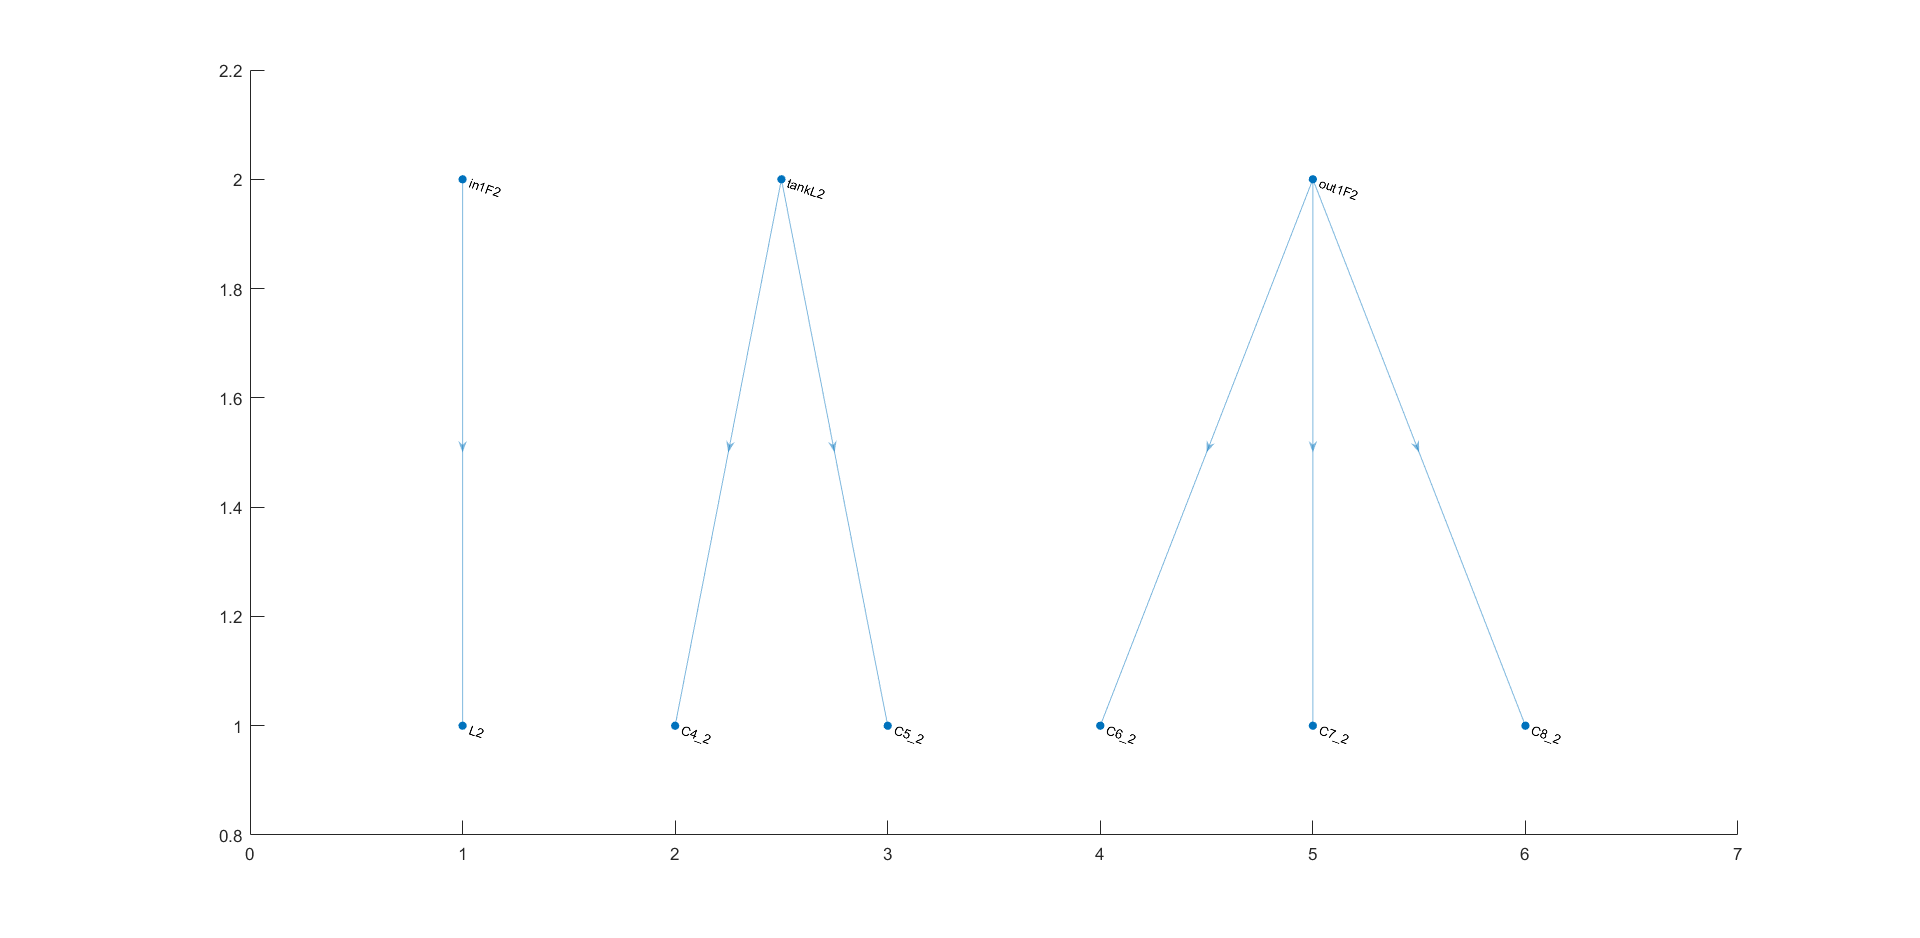
\includegraphics[width=\textwidth]{bilder/04_code_Modul2_Error.png}
\caption[fehlerhafter Digraph von Modul 2]{Digraph von Modul 2 auf Basis der HAZOP mit syntaktischen Abweichungen}
\label{fig:graph_mod2Error}
\end{figure}

Entspricht die Syntax aller drei Module den Erwartungen, so kann ein Graph mit drei Subgraphen geniert werden, welcher in \figref{fig:graph_sysGes} abgebildet ist. Die Module 1 und 2 weisen in diesem Fall jeweils eine Kopplung vom Eingangsstrom \"uber das Tankvolumen zum Ausgangsstrom auf. Das in \figref{fig:PIDMod3} dargestellte dritte Modul besteht aus drei Teilgraphen. Es weist entsprechend der in \tabref{tab:hazopBsp_M3} dargestellten \ac{hazop} keine Wechselwirkung zwischen den betrachteten Prozessgr\"o\ss{}en auf. Die Kopplung der drei Module wird im folgenden Abschnitt \ref{sec:kopplung} erl\"autert.

\begin{figure}[h!tb]
\centering
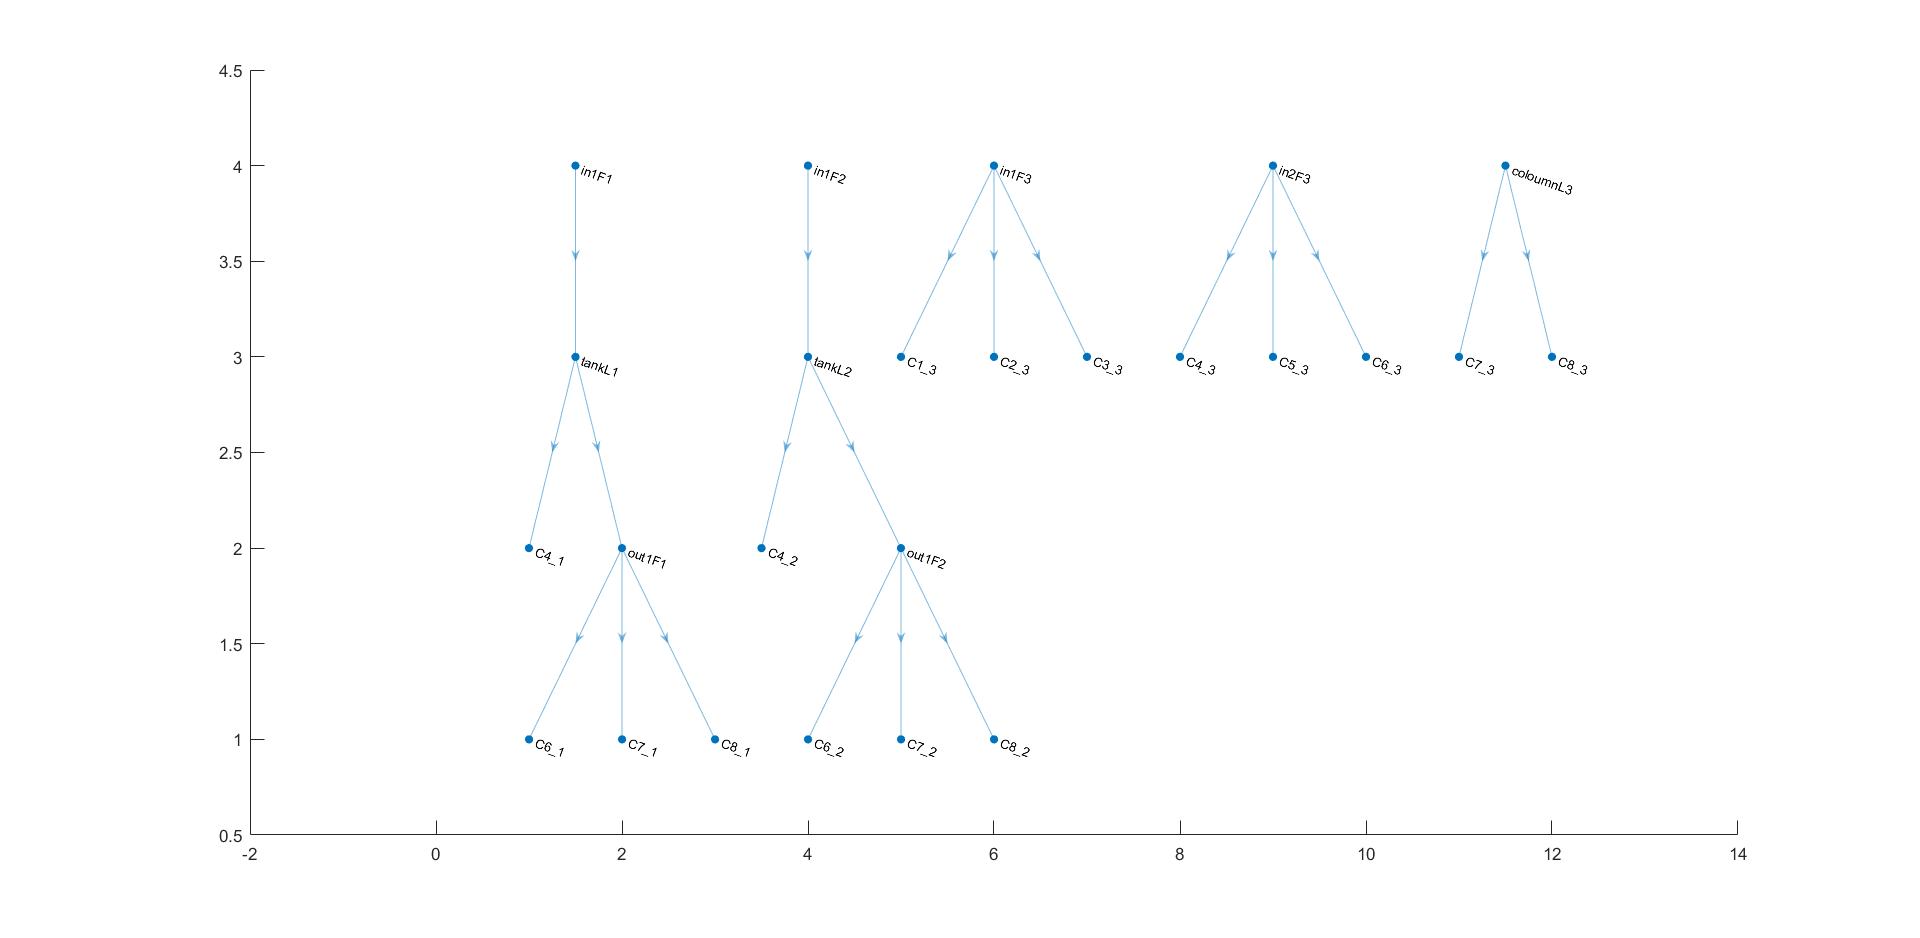
\includegraphics[width=\textwidth]{bilder/04_code_Sys1.png}
\caption[Digraphen aller Module]{Digraph vom Gesamtsystem mit korrekter Syntax der HAZOP}
\label{fig:graph_sysGes}
\end{figure}

\section{Kopplung von Graphen und Fehlerfortpflanzung}\label{sec:kopplung}
Anhand der \ac{hazop} von einzelnen Modulen k\"onnen entsprechend dem im Abschnitt \ref{sec:graphHazop} beschriebenen Algorithmus gerichtete Graphen erzeugt werden, welche die in der \ac{hazop} enthaltenen Informationen widerspiegeln. Wird eine Anlage aus Modulen zu einer Gesamtanlage kombiniert, so enth\"alt das \ac{pid} der Gesamtanlage die notwendigen Informationen, um die Kopplung der Module zu beschreiben. Diese Informationen sind \figref{fig:PIDGes} zu entnehmen. \newline
Die physische Kopplung von Modulen erfolgt durch Einsatz von Rohren. Die Funktion \glqq connectPipe\grqq { }ist daher der Funktionsweise eines Rohres nachempfunden. Innerhalb eines Rohres kann es bez\"uglich des Durchflusses zu Abweichungen kommen. Ursache daf\"ur k\"onnen Lecks oder Hindernisse im Rohr sein. Weiterhin kann ein Rohr als passive Komponente keine Abweichungen kompensieren sondern es leitet diese an angrenzende Module weiter. Die Verbindung von zwei Modulen wird durch Einf\"uhrung eines neuen Knoten symbolisiert, welcher Abweichungen bez\"uglich eines Stoffstromes vom Vorg\"angermodul an das Nachfolgemodul weiterleitet. In \figref{fig:graph_sysGesVerb} ist die Gesamtanlage dargestellt. Die Module 1 und 2 wurden dabei  mit Hilfe der beschriebenen Funktion \glqq connectPipe\grqq { } unter expliziter Angabe der Knoten verbunden. 

\begin{figure}[h!tb]
\centering
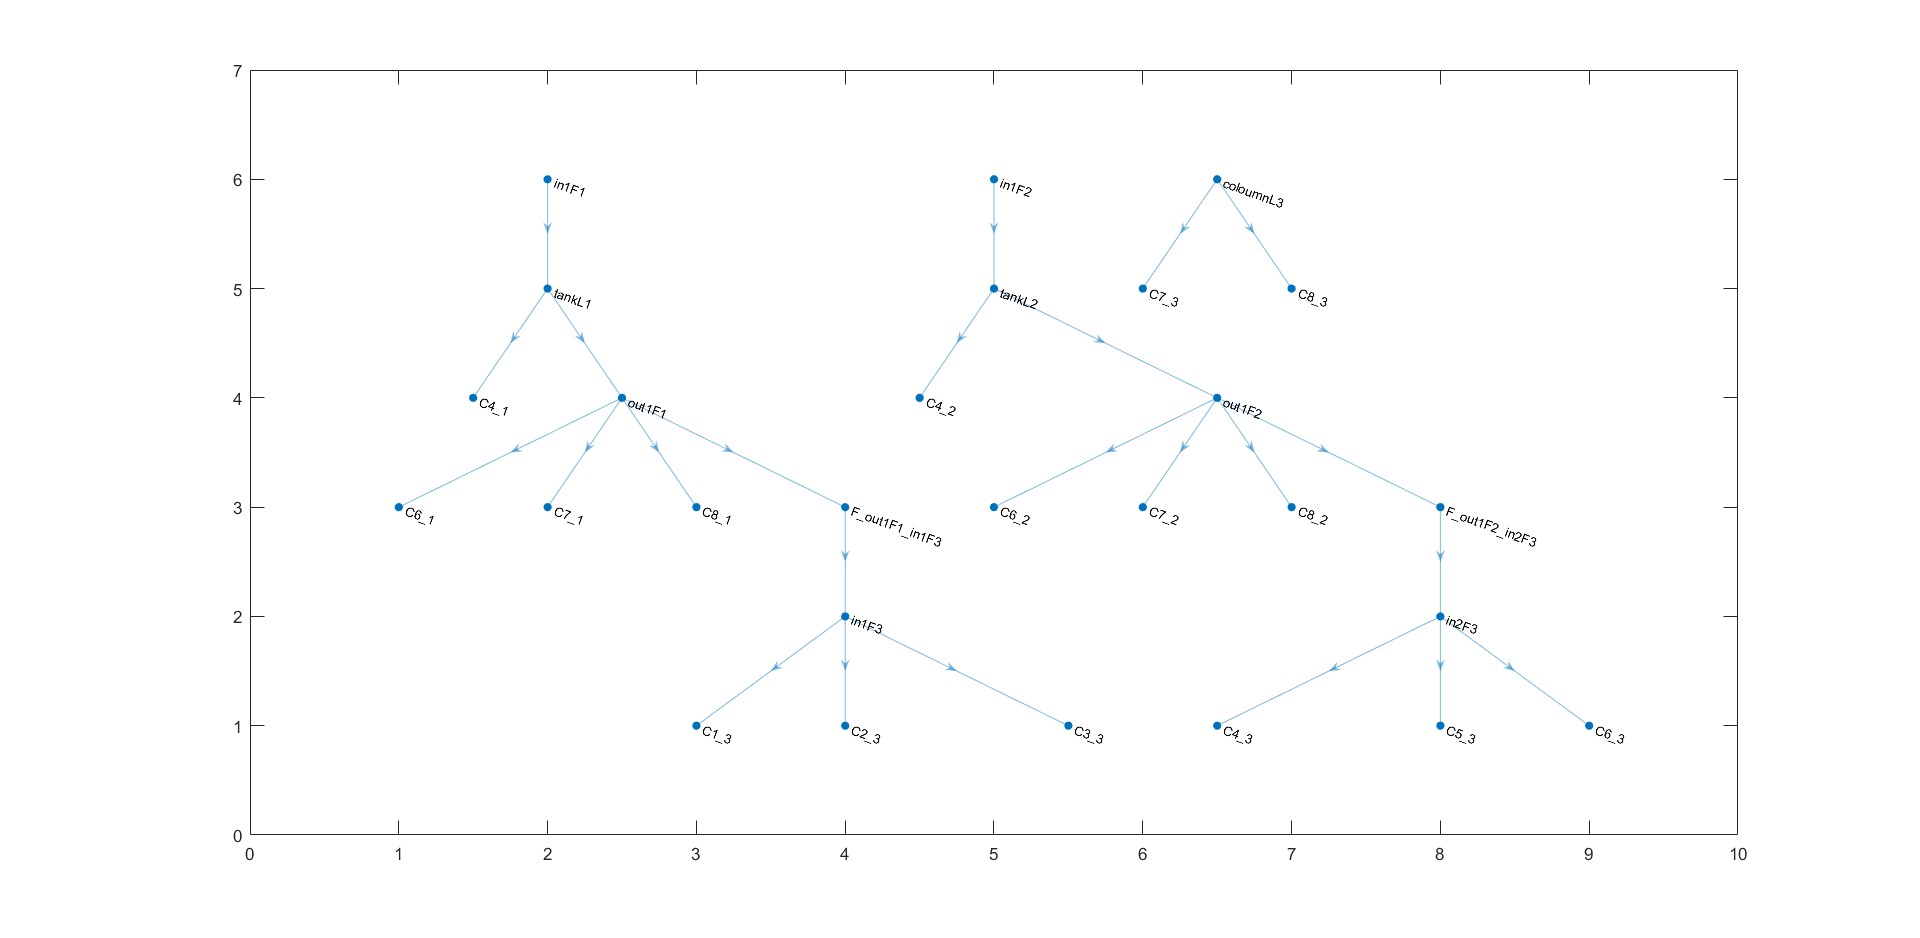
\includegraphics[width=\textwidth]{bilder/04_code_Sys2.png}
\caption[Digraph gekoppeltes Gesamtsystems]{Digraph vom Gesamtsystem mit verbundenen Modulen}
\label{fig:graph_sysGesVerb}
\end{figure}

Dieser gerichtete Graph kann durch Anwendung geeigneter Algorithmen auf die Fortpflanzung von Fehlern untersucht werden. Dazu wird im ersten Schritt ein Knoten festgelegt, dessen Auswirkungen auf den Gesamtprozess durch Abweichung des symbolisierten Parameters ermittelt werden soll. Mit Hilfe einer Tiefenanalyse k\"onnen alle Knoten ermittelt werden, welche ohne mehrfache Schleifen unter Beachtung der Richtung der Kanten mit diesem Konten verbunden sind. Die so erhaltenen Knoten k\"onnen als Untergraph dargestellt werden. In \figref{fig:graph_sysGesFehlerfort} ist das Ergebnis aller m\"oglichen Abweichungen von \textit{tankL1} auf den restlichen Prozess dargestellt. Dabei ist aber noch nicht untersucht, ob diese Fortpflanzung sinnvoll ist. F\"ur den Untergraphen muss an jedem Knoten untersucht werden, ob die am Vorg\"angerknoten erzeugte Auswirkung einer g\"ultigen Abweichung des betrachteten Knotens entspricht und ob die Abweichungen des aktuell betrachteten Knotens durch Auswirkungen des Vorg\"angerknotens entstehen k\"onnen. Betrachtet man den Knoten \textit{out1F1} so stellt man fest, dass die Abweichungen \textit{more flow} und \textit{reverse flow} nicht als Auswirkung einer Abweichung von \textit{tankL1} entstehen k\"onnen. Die Verbindungen zu den entsprechenden Auswirkungsknoten \textit{C7{\_}1} und \textit{C8{\_}1} sind daher im Rahmen der Fehlerfortpflanzungsanalyse ung\"ultig. Die Abweichung \textit{less level} von \textit{tankL1} kann sich jedoch in das Modul 3 fortpflanzen und dort die Auswirkung mit der $\text{ID} = 3$ \textit{changed reaction balance} erzeugen. 

\begin{figure}[h!tb]
\centering
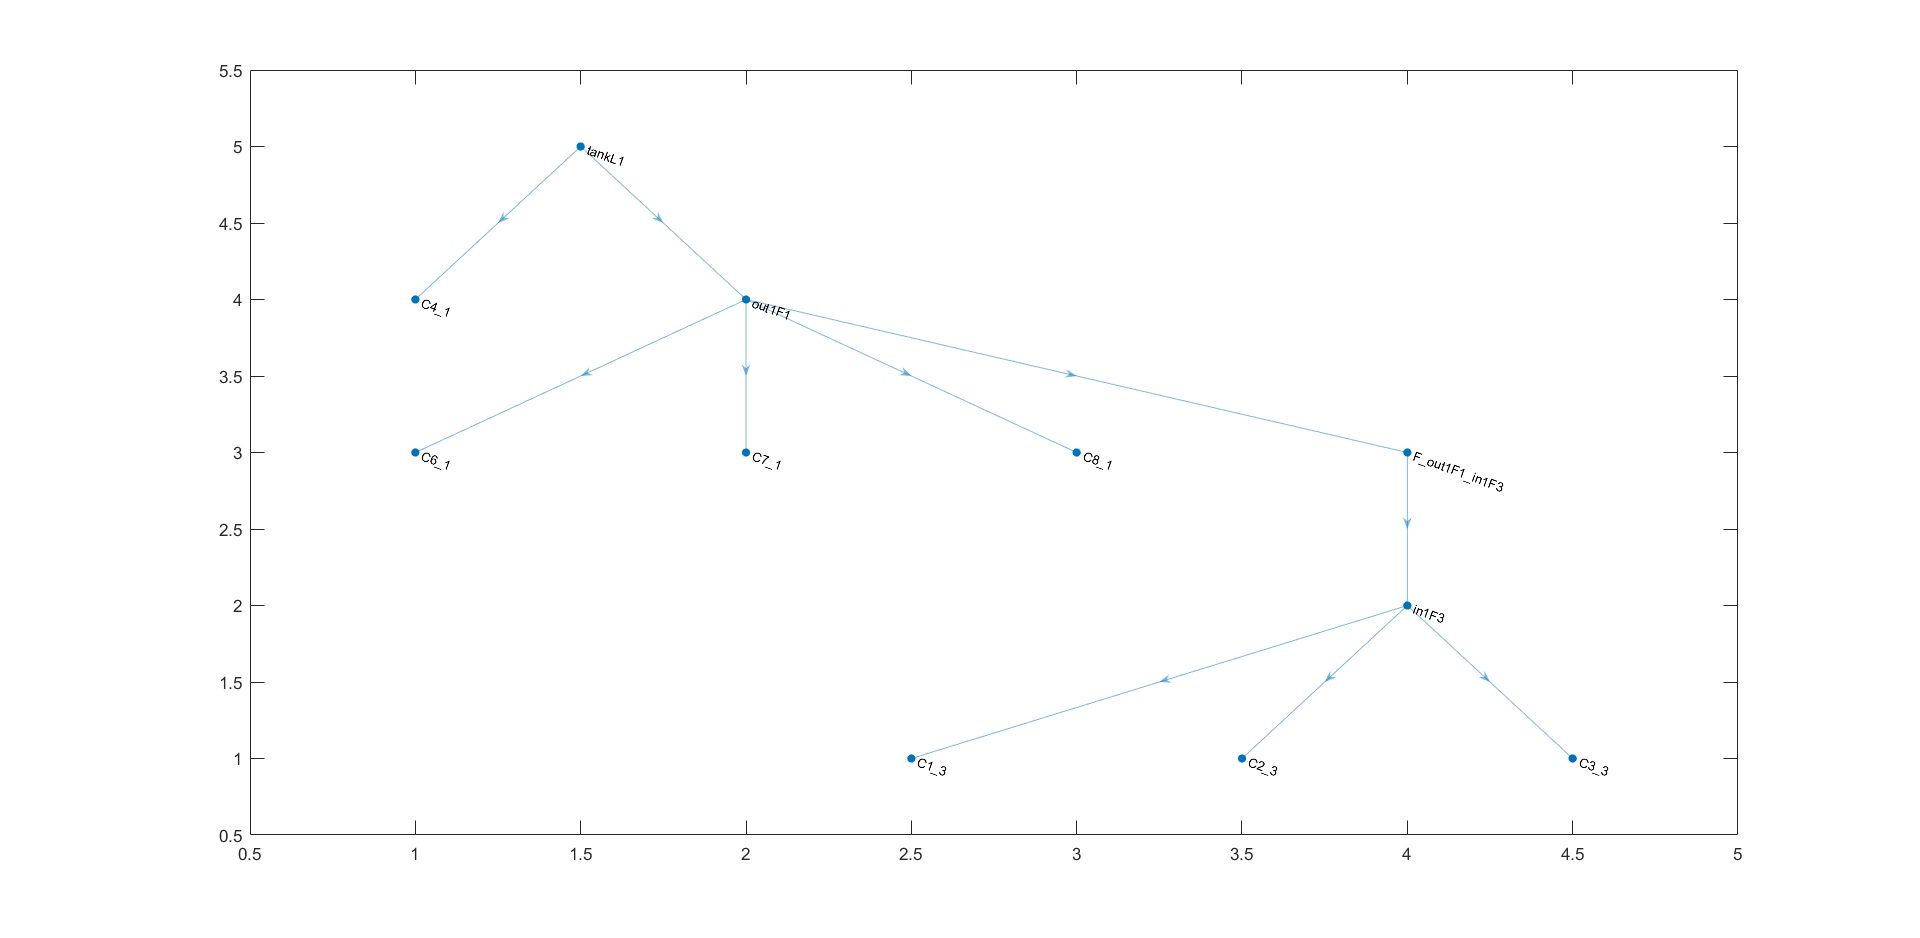
\includegraphics[width=\textwidth]{bilder/04_code_Sys2TankL1FF.png}
\caption[Fehlerfortpflanzung im Gesamtsystem]{Auswirkung einer Abweichung des F\"ullstandes im Tank von Modul 1 auf das Gesamtsystem}
\label{fig:graph_sysGesFehlerfort}
\end{figure}

Auf Basis der \acp{hazop} einzelner Module und einem \ac{pid} der Gesamtanlage kann demnach teilautomatisiert ein Graph erzeugt werden, anhand dessen man die Fortpflanzung von Fehlern untersuchen kann. Aussagen dar\"uber, ob die derart ermittelten Fehler in einem Modul erkannt und beherrscht werden k\"onnen sind derzeit nicht m\"oglich, da zum entwickeln eines geeigneten Algorithmus die Festlegung einer Ontologie erforderlich ist. Ohne Festlegung einer Ontologie m\"usste eine Syntax definiert werden, mit Hilfe derer die notwendigen Informationen dargestellt werden. Wie im Abschnitt \ref{sec:graphHazop} gezeigt wird ist dieses Vorgehen bei komplexen, textuell basierten Informationen jedoch sehr fehleranf\"allig. Weiterhin ist die Datenbasis um derartige komplexe Untersuchungen durchzuf\"uhren derzeit zu gering. 